\section{Theorie}\label{sec:theorie}
Nachdem zunächst auf den Grundlegenden Aufbau eines Lasers und die Einzelheiten des Entstehungsprozesses von Laserstrahlung und relevante charakteristische Eigenschaften der Wellen eingegangen wird, folgt mit diesem Wissen eine Einführung in die Funktionsweise des verwendeten \ce{He}-\ce{Ne}-Lasers.
\subsection{Aufbau eines Lasers}
Im wesentlichen besteht ein Laser aus drei Komponenten: dem \textbf{aktiven Medium}, der (selektiven) \textbf{Energiepumpe} und dem \textbf{Resonator}.\\
Das Aktive Medium ist ein Material, welches unter speziellen Vorraussetzungen die Fähigkeit besitzt, die Intensität von durchlaufendem Licht zu verstärken. Dies geschieht, da Atome in solchen Konfigurationen angeregt werden, die induzierte Emission von Photonen wahrscheinlicher als Absorption für bestimmte Frequenzen werden lassen(siehe \hyperref[subsec:entstehung]{Entstehung von Laserstrahlung}).\\
Die Energiepumpe liefert die nötige Energie um die Atome in die gewünschten angeregten Zustände zu heben. Erst durch sie kann der Laserbetrieb ermöglicht werden.\\
Der Resonator, typischerweise bestehend aus zwei Spiegeln, sorgt dafür, dass das Licht mehrmals das aktive Medium durchläuft indem er es hin- und herreflektiert. So kann die Verstärkung der Intensität signifikant genutzt werden, um einen stabilen Strahl zu konstruieren. Diese Energie des Laserstrahls wird zu einem großen Teil im Resonator in wenigen Resonatormoden gespeichert, was zu einer hohen Strahlungsdichte in ausgewählten Wellenlängen führt.\cite{Demtroeder} 
\subsection{Entstehung von Laserstrahlung}\label{subsec:entstehung}
Durch die dem System mittels der Pumpe hinzugeführte Energie werden die Atome des aktiven Mediums von ihrem Grundzustand in verschiedene höher gelegene Energieniveaus gehoben.
Sei etwa $k$ ein energetisch höherer quantenmechanischer Zustand des Atoms als ein mit ihm durch einen erlaubten Übergang verbundener Zustand $i$, so würde im thermischen Gleichgewicht für die Besetzungszahlen der Zustände $N_i>N_k$ gelten. Die erwähnte selektive Energiezufuhr führt nun dazu, dass wie in \autoref{fig:inversion} dargestellt, sich die Besetzungsverteilung verändert, es tritt \textbf{Besetzungsinversion} auf.
\begin{figure}[H]
    \centering
    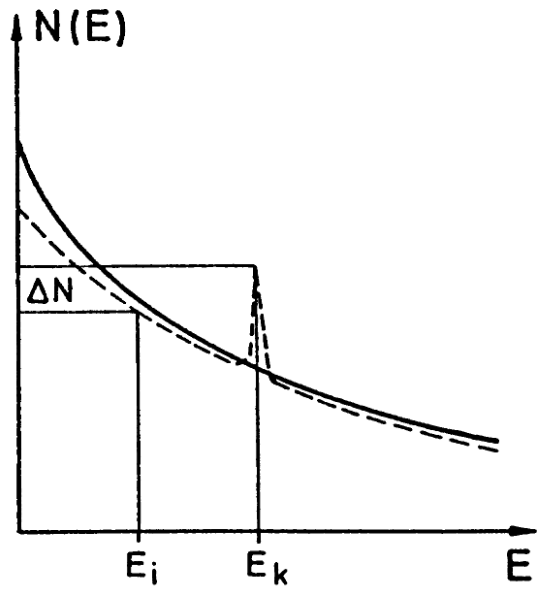
\includegraphics[scale=0.5]{Ressourcen/inversion.png}
    \caption{Thermische Besetzungsverteilung (durchgezogen) und Inversion (gestrichelt)\cite{Demtroeder}}\label{fig:inversion}
\end{figure}
Trifft ein Photon der Frequenz $\nu = \frac{E_k-E_i}{h}$ auf ein angeregtes Atom oder Molekül der Energie $E_k$, so kann es dieses dazu veranlassen in den tieferen Zustand $E_i$ überzugehen unter Emission eines Photons derselben Frequenz und Richtung.
So kann durch die Besetzungsinversion die Wahrscheinlichkeit für induzierte Emission die der Absorption durch das Medium übersteigen, wie durch
\begin{align}
    N_kB_{ki}\rho(\nu)>N_iB_{ik}\rho(\nu)
\end{align}
beschrieben wird. Hierbei sind $B$ die Einstein-Koeffizienten der Zustandsübergänge und $\rho$ ist die Strahlungsdichte in Abhängigkeit der Frequenz bzw Mode innerhalb des Resonators. So kann durch fokussierung der Energie in wenigen Resonatormoden die induzierte Emission wesentlich größer werden als die Absorption und das Licht erfährt eine Verstärkung bei durchlauf des aktiven Mediums.
Für die Intensität der Strahlung bei eintrittstiefe $z$ innerhalb des Mediums gilt
\begin{align}
    I(\nu,z) = I(\nu,z=0)\cdot\exp{-\alpha(\nu)z}\text{,}
\end{align}
mit dem Absorptionskoeffizient 
\begin{align}
    \alpha(\nu)=(N_i-\frac{g_i}{g_k}N_k)\sigma(\nu)\text{,}\label{eqn:alpha}
\end{align}
der wiederum von den Besetzungszahlen, den statistischen Gewichten $g$ und dem optischen Absorptionsquerschnitt $\sigma$ des Übergangs $E_i \rightarrow E_k$ bestimmt wird.
Werden nun noch die verschiedenen Verluste durch Reflexion, Absorption in den einschließenden Fenstern des Mediums, Beugung und Streuung unter der Beschreibung $(\frac{I}{I_0})_\text{passiv} = \exp{-\gamma}$ für einen Durchgang miteinbezogen, so ergibt sich konkret für ein Medium der länge $L$ ein Verstärkungsfaktor
\begin{align}
    G= \left(\frac{I}{I_0}\right)_\text{aktiv}=\exp{-2\alpha(\nu)L-\gamma}\text{.}\label{eqn:G}
\end{align}
und somit unter Verwendung von \autoref{eqn:alpha} die Schwellwertbedinung für Laserbetrieb
\begin{align}
    \Delta N = N_k\frac{g_i}{g_k}-N_i>\Delta N_S = \frac{\gamma}{2\sigma(\nu)L}\text{.}
\end{align}
Für den Fall dass die tatsächliche Inversion die Schwellwertinversion $\Delta N_S$ übersteigt wird die Intensität solange anwachsen bis durch die hohe induzierte Emissionsrate $N_k$ so weit reduziert wird bis sich Sättigung in Form von $\Delta N = \Delta N_S$ einstellt.

Mithilfe der Bilanzgleichungen der modellischen Zustände $1$ und $2$
\begin{align*}
    \frac{dN_1}{dt} &= (N_2 - N_1) B_{21} n h \nu + N_2 A_{21} - N_1 R_1 \\
    \frac{dN_2}{dt} &= P - (N_2 - N_1) B_{21} n h \nu - N_2 A_{21} - N_2 R_1 \\
    \frac{dn}{dt}   &= -\beta n + (N_2 - N_1) B_{21} n h \nu\text{,}
\end{align*}
wobei $P$ die Pumpleistung, $A$ und $B$ die spontane, beziehungsweise induzierte Emission, $R$ die Relaxation und $\beta$ den Verlustfaktor der Energie einer Resonatormode in Abwesenheit des aktiven Mediums beschreibt, lassen sich die Zusammenhänge im stationären Betrieb $P=N_1R_1+N_2R_2=\beta n + N_2(A_{21}+R2)$ klarmachen.
Speziell ergibt sich für den Verlustexponenten
\begin{align}
    \gamma = \beta T = \beta \frac{2L}{c}\label{eqn:gamma}
\end{align}
und aus der Beschreibung des stationären Betriebs, dass kontinuierliche Laserstrahlung nur für eine effektive Lebensdauer des Zustands $1$ resultiert, welche kleiner als $\frac{1}{A_{21}+B_{21}\rho}$ ist.
Zusätzlich lässt sich aus der letzten Bilanzgleichung, der Vorraussetzung $\frac{\mathrm{d} n}{\mathrm{d} t}=0$ und \autoref{eqn:gamma} mit einiger zusätzlicher Theorie erneut die oben erwähnte Schwellwertbedinung herleiten.

Da sich in einem allgemeinen Holraumresonator die Strahlungsenergie auf alle Moden entsprechend dem thermischen Gleichgewicht verteilen würde, entfallen respektiv weniger Photon auf eine einzelne Eigenmode, was ungeeignet für einen Laserresonator ist.
Die erwünschte hohe Konzentration und somit starke Rückkopplung der Strahlung für wenige Moden kann somit dadurch erreicht werden, dass in andere Moden emittierte Energien weitaus schlechter im Resonator reflektiert werden, beziehungsweise einen hohen relativen Energieverlust $\mathrm(d)W_k=-\beta_kW_k\mathrm(d)t$ besitzen.
Daraus folgt die Resonatorgüte
\begin{align}
    Q_k=-2\pi\nu \frac{W_k}{\dot{W}_k}=2\pi\nu\tau_k\text{,}
\end{align}
mit der mittleren Verweilzeit $tau_k$ einer Mode im Resonator, welche den Energieverlust einer Mode pro Periode $\frac{1}{\nu}$ angibt.
Um dafür zu sorgen dass die Pumpenergie und somit die Strahlungsenergie des aktiven Mediums bevorzugt in wenigen Moden speichert, muss der Resonator folgend so beschaffen sein, dass er für wenige Moden kleine Verlustfaktoren $\beta_k$, für alle anderen aber große Verluste aufweist und die Wahrscheinlichkeit für induzierte Emission in diesen wenigen Moden größer wird.

Der offene Resonator, bestehend aus zwei Spiegeln und offen in andere Richtungen wirkt durch seine Geometrie restriktiv auf die Richtung des Lichts und erfüllt somit die eben genannten Eigenschaften zur Modenselektion.
Dadurch dass der Spiegelabstand $d$ oft groß gegenüber dem nutzbaren Durchmesser der Spiegel ist, treten wesentliche Beugungsverluste auf. Zusätzlich zum Verlust durch Transmission an den Spiegeln $\gamma_R=\ln{R_1R_2}$ muss nun auch der Beugungsverlust $\gamma_B$ betrachtet werden.
Es lässt sich zeigen, dass mithilfe der Fresnel-Zahl $F_N=\frac{a^2}{\lambda d}$, wobei $a$ der Radius des Spiegels und $\lambda$ die Wellenlänge des betrachteten Laserlichts ist, sich der Verlustexponent für Beugung als
\begin{align}
    \gamma_B=\frac{1}{F_N}
\end{align}
bestimmen lässt. Die Fresnel-Zahl gibt an, wie viele Fresnelzonen auf einem Resonatorspiegel entstehen.
\subsection{Eigenschaften von Laserstrahlung}\label{subsec:eigenschaften}
Es folgt eine kurze Einführung in die Modenstruktur des offenen Resonators. Anschließend wird auf die Stabilitätskriterien eingegangen und das Freqzensspektrum dargestellt.
\subsubsection{Modenstruktur}
Wegen unterschiedlichen Beugungsverlusten abhängig vom Abstand zum Spiegelmittelpunkt können ebene Wellen im offenen Resonator nicht zu stationären Feldverteilungen führen. Eine solche stellt sich durch Überlagerung aller Reflektierten Wellen erst dann ein, wenn sich die räumliche Feldstärkeverteilung über den Resonatorquerschnitt nicht mehr ändert, die absolute Energie kann abhängig von der Pumpleistung jedoch variieren. Diese Verteilungen sind das Analogon zu den Moden des geschlossenen Resonators, den ebenen Wellen.
\begin{figure}[H]
    \centering
    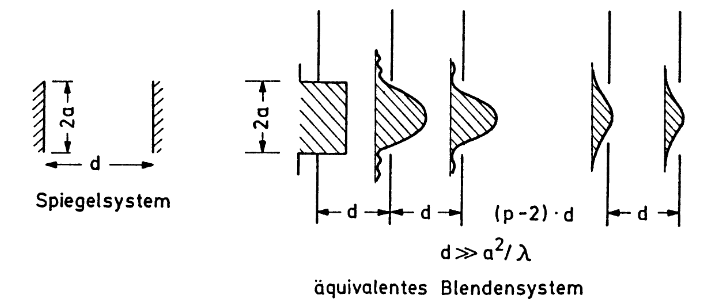
\includegraphics[scale=0.7]{Ressourcen/kette.png}
    \caption{Skizze zur Äquivalenz der zwei optischen Aufbauten\cite{Demtroeder}}\label{fig:kette}
\end{figure}
Wird mittels eines iterativen Verfahrens basierend auf der Kirchhoff-Fresnel'schen Beugungstheorie der Resonator als eine Lochblenden-Kette  wie in \autoref{fig:kette} modelliert, so ergibt sich für die Amplitude der Elektromagnetischen Strahlung in eine Ebene bei beliebigem $z$ Wert
\begin{align}
    A_\text{mn}(x,y,z)=C_\text{mn}H_\text{m}(x^*)H_\text{n}(y^*)\exp{\left(-\frac{{x^*}^2+{y^*}^2}{4}\right)}\exp{(-i\phi)}\text{.}
\end{align}
Hierbei beschreiben $m$ und $n$ die Anzahl der Knotenlinien in x bzw y-Richtung, $C$ einen Normierungsfaktor, $H_\text{k}$ das Hermitischen Polynom $k$-ter Ordnung, $\phi$ die Phase, $x^*=\sqrt{2}\frac{x}{w}$ und $y^*=\sqrt{2}\frac{y}{w}$ sind normierte Koordinaten und $w(z)=\sqrt{\lambda\frac{d}{2\pi}{\left[1+\left(\frac{2z}{d}\right)^2\right]}}$ ein Maß für die radiale Abhängigkeit. Die Phase ist hinsichtlich der Messbaren Intensität $I\propto|A_\text{mn}|^2$ an dieser Stelle nicht von Bedeutung.
\begin{figure}[H]
    \centering
    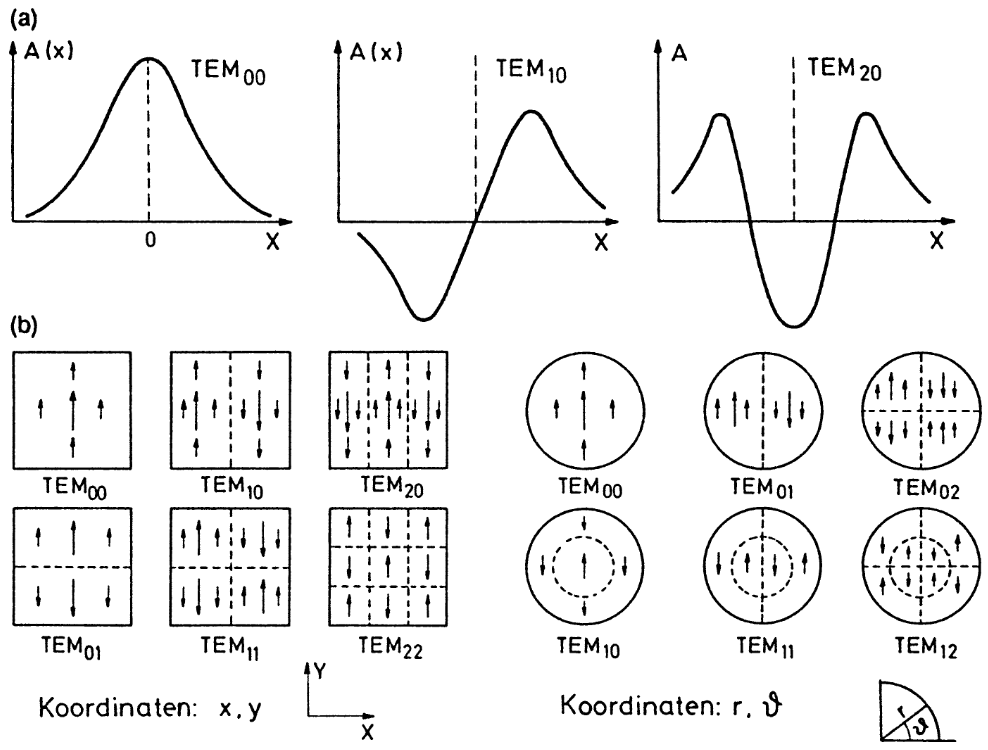
\includegraphics[scale=0.5]{Ressourcen/moden.png}
    \caption{\textbf{(a)} Amplitudenprofil in x-Richtung \textbf{(b)} Zweidimensionale Amplitudenverteilung in verschiedenen Koordinatensystemen\cite{Demtroeder}}\label{fig:moden}
\end{figure}
Eine Auswahl dieser Moden ist in \autoref{fig:moden} dargestellt, beginnend mit der Fundamentalmode $\mathrm{TEM_{00}}$. Diese ist aufgrund ihrer Radialsymmetrie auch eine Axiale Mode.
\subsubsection{Stabilität}
Wie im vorherigen Abschnitt erwähnt sollten für eine Stabile Funktion des Lasers die Spiegel die Feldverteilung bei Reflektion bis auf einen Gesamtverlust reproduzieren. Wird ein Strahl mit einem Gaußförmigen Intensitätsprofil unter der Bedingung dass dieser nach einem Umlauf sich nicht ändert, ergeben sich die Formeln
\begin{align*}
    \pi w_1^2 &=\lambda d \sqrt{\frac{g_1}{g_1(1-g_1g_2)}}\\
    \pi w_2^2 &=\lambda d \sqrt{\frac{g_2}{g_2(1-g_1g_2)}}
\end{align*} 
mit der Abkürzung 
\begin{align}
    g_i=1-\frac{d}{b_i}
\end{align} 
für die Fleckgrößen des Gaußradius $w$ auf den zwei Spiegeln. $b$ beschreibt hier den Krümmungsradius des jeweiligen Spiegels.
Aus den Formeln sind die Stabilitätsbedingungen
\begin{align}
    &0<g_1g_2<1\text{ oder}\\
    &g_1=g_2=0
\end{align}
ersichtlich. In \autoref{tab:stabil} sind einige Resontortypen inklusive ihrer Spiegelradien $b$ und der erwähnten Stabilitätsparametern $g$ aufgeführt.
\begin{table}[H]
  \centering
  \caption{Resonatortypen und ihre Eigenschaften}
  \begin{tabular}{l | l | l}
    \toprule
    Typ & Spiegelradien & Stab. Parameter \\
    \midrule
    konfokal ($b_1 \neq b_2$)            & $b_1 + b_2 = 2d$             & $g_1 + g_2 = 2g_1g_2$ \\
    konzentrisch                         & $b_1 + b_2 = d$              & $g_1 \cdot g_2 = 1$ \\
    symmetrisch                          & $b_1 = b_2$                  & $g_1 = g_2 = g < 1$ \\
    symmetrisch konfokal                 & $b_1 = b_2 = d$              & $g_1 = g_2 = 0$ \\
    symmetrisch konzentrisch             & $b_1 = b_2 = \frac{1}{2}d$   & $g_1 = g_2 = -1$ \\
    semikonfokal                         & $b_1 = \infty, b_2 = 2d$     & $g_1 = 1, g_2 = \frac{1}{2}$ \\
    eben                                 & $b_1 = b_2 = \infty$         & $g_1 = g_2 = +1$ \\
    \bottomrule
  \end{tabular}
  \label{tab:stabil}
\end{table}
\subsubsection{Frequenzspektrum}
Bei kontinuierlicher Erhöhung der Pumpleistung wird die Schwellwertinversion zuerst für die Frequenzen erreicht, für die \autoref{eqn:G} maxmial wird.
Da aber wie oben erläutert der Verlustexponent $\gamma$ von der Resonatorbeschaffenheit abhängt, ist somit auch das Frequenzspektrum abhängig vom Modenspektrum.
Für gasförmige Lasermedien im sichtbaren Spektrum ist das Verstärkungsprofil $\alpha$ durch ein Doppler-Profil 
\begin{align}
    \alpha(\nu)=\alpha(\nu_0)\exp{\left[-\left(\frac{1.66(\nu-\nu_0)}{\Delta\nu_D}\right)\right]}
\end{align}
beschrieben. Dies ist in \autoref{fig:alpha} zusammen mit den Eigenfrequenzen der longitudinalen Lasermoden dargestellt. Ausgehend von der einfachen Bedingung an die Länge des Resonators $L = N\cdot\frac{\lambda}{2}$ mit $N\in\mathbb{N}$ lassen sich die Abstände zwischen diesen als $\delta\nu=\frac{c}{2d}$ bestimmen.
\begin{figure}[H]
    \centering
    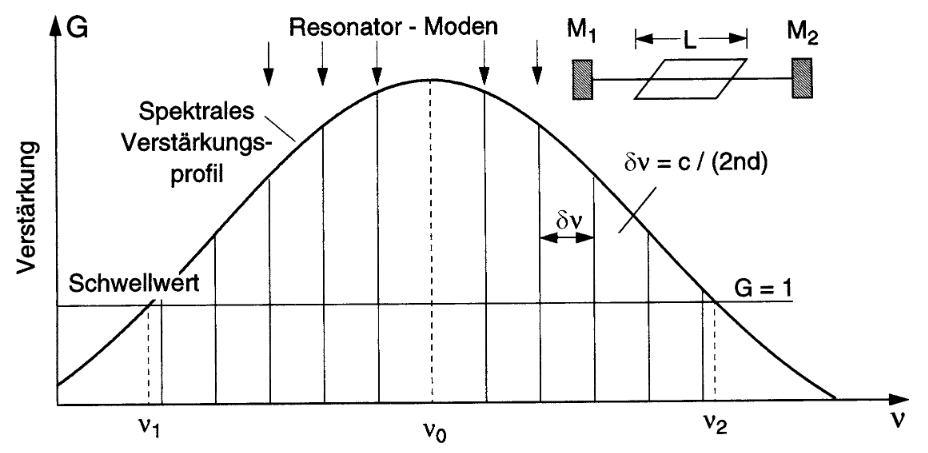
\includegraphics[scale=0.5]{Ressourcen/alpha.png}
    \caption{Schematischer Plot der Verstärkung eines Lasers und den erlaubten Moden oberhalb des Schwellwerts\cite{Demtroeder}}\label{fig:alpha}
\end{figure}
Als letzten Schritt kann nun die Nettoverstärkung unter Berücksichtigung der Frequenzabhängigen Verluste aufgetragen werden, wie in \autoref{fig:netto} zu sehen. Logischerweise kann stabile Lasertätigkeit nur für Verstärkungen oberhalb der Schwellwertgerade $G=1$ einsetzen.
\begin{figure}[H]
    \centering
    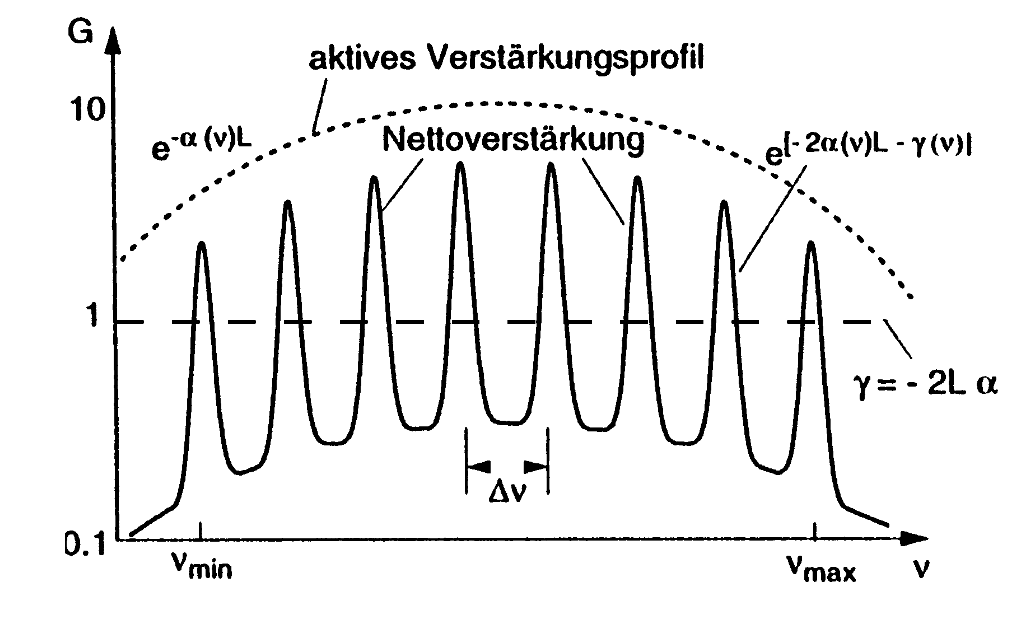
\includegraphics[scale=0.4]{Ressourcen/netto.png}
    \caption{Nettoverstärkung des Verstärkungsprofils $\alpha$ inklusive Schwellwertgerade\cite{Demtroeder}}\label{fig:netto}
\end{figure}
\subsection{Funktionsweise eines He-Ne-Lasers}
Aufbauend auf dem Niveauschema für \ce{He}-\ce{Ne}-Gase erfolgt eine Erklärung der spezifischen Operation des zugehörigen Lasers.
\subsubsection{Niveauschema}
Wie in \autoref{subsec:entstehung} beschrieben werden die Atome des aktiven Mediums durch äußere Energiezufuhr in höhere Energiezustände gehoben und für Lasertätigkeit muss anschließend Besetzungsinversion vorliegen.
Konkret für den im Versuch betrachteten Laser sind mögliche Übergänge der Atome in \autoref{fig:niveau} skizziert.
\begin{figure}[H]
    \centering
    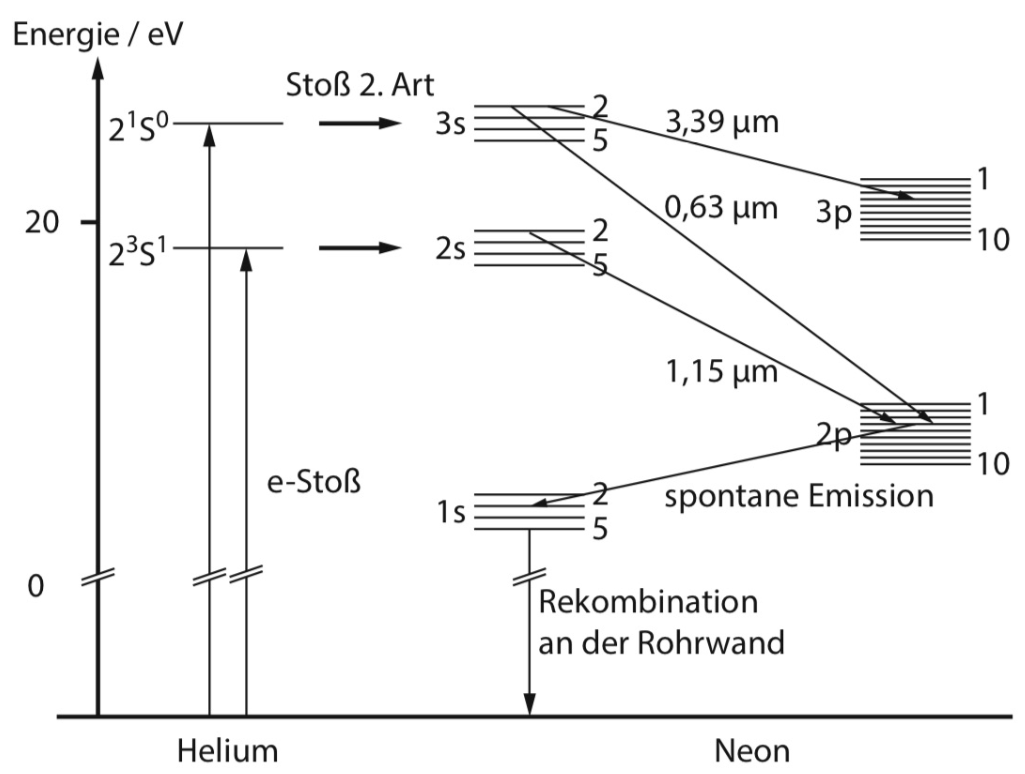
\includegraphics[scale=0.4]{Ressourcen/niveau.png}
    \caption{Termschema des He-Ne-Lasers\cite{eichler}}\label{fig:niveau}
\end{figure}
Durch eine Gasentladung und subsequente Elektronenstöße werden Heliumatome in Metastabile zustände \ce{He^*} angeregt und übertragen diese Energie mittels eines Stoßes 2. Art 
\begin{align}
  \text{He}^* + \text{Ne} \rightarrow \text{He} + \text{Ne}^* + \Delta E
\end{align}
auf das Neonatom. So koppelt der beinahe gefüllte Rumpf $\mathrm{1s^22s^22p^5}$ mit einem sogenannten Leuchtelektron höherer Energie, etwa $\mathrm{3s}$. In der Abbildung werden Termbezeichnungen nach Paschen für Neon angenommen.
Die Selektivität der Anregung der höheren Zustände profitiert von den langen Lebensdauern der metastabilen Helium-Zustände, da diese dichter auftreten.
Am relevantesten für den vorliegenden Versuch ist der rote Übergang mit der Wellenlänge $\lambda=\SI{633}{\nano\meter}$. Beginnend mit dem Übergang $\mathrm{3s^2\rightarrow2p^4}$ zerfällt das untere Niveau unter sponater Emission zu $\mathrm{1s^3}$, welcher hinsichtlich der relevanten Zerfallsmechanismen stabil ist. So kann es passieren, dass dieser Zustand erneut durch Stöße in 2p-Niveaus gehoben wird, die Gesamtanzahl der Atome auf diesem Energieniveau somit erhöht und letzendlich die Besetzungsinversion schmälert.
Deshalb ist eine schnelle Rekombination an der Rohrwand essentiell für den Versuch, um die 1s Zustände abzugreifen und der Wirkungsgrad ist abhängig vom Rohrdurchmesser.
\subsubsection{Operation eines He-Ne-Lasers}
Das Grundsätzliche Prinzip des in \autoref{fig:henelaser} skizzierten \ce{He}-\ce{Ne}-Laser ist wie im vorherigen Unterabschnitt erwähnt die Gasentladung des \ce{He}-\ce{Ne}-Gases.
\begin{figure}[H]
    \centering
    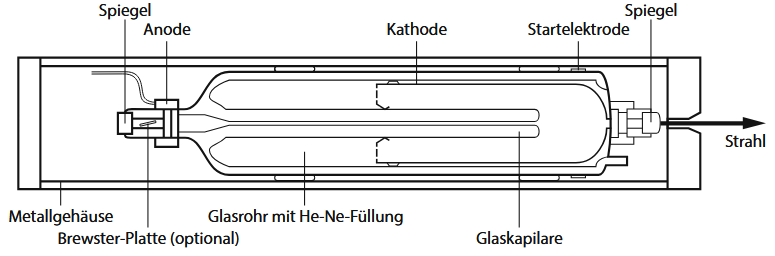
\includegraphics[scale=0.7]{Ressourcen/henelaser.png}
    \caption{Querschnitt mit elementaren Bestandteilen eines \ce{He}-\ce{Ne}-Lasers\cite{eichler}}\label{fig:henelaser}
\end{figure}
Da das Verhältniss von induzierter Emission zu spontaner Emission mit kleineren Frequenzen zunimmt, sind für eine stabile Lasertätigkeit bei \SI{633}{\nano\meter} selektive Bauelemente nötig.
So etwa auch die Brewsterfenster an dem Entladungsrohr, welche die viel prominentere Infrarot-Schwingung unterdrückt und das zur Einfallsebene parallel polarisierte Licht nicht durch Reflexion geschwächt wird. So schwingt der Laser nur in der Mode der respektiven Polarisationsrichtung.
Im Normalbetrieb wird der Laser in der $\mathrm{TEM_{00}}$ Mode schwingen, wobei auch andere Moden bei geschickter Unterdrückung erreichbar sind. Bei Raumtemperatur beträgt die Dopplerbreite des Hauptübergangs \SI{1500}{\mega\hertz}, welche für eine beispielhafte Resonatorlänge von $d=\SI{30}{\centi\meter}$ nur drei axiale Moden gleichzeitig innerhalb der Doppler-verbreiterten Linie zulassen würde.